\documentclass{article}
\usepackage[utf8]{inputenc}

\newcommand{\ii}{{\bf i}}
\newcommand{\jj}{{\bf j}}
\newcommand{\kk}{{\bf k}}
\newcommand{\id}{{\bf 1}}
\newcommand{\hur}{\frac{\id+\ii+\jj+\kk}{2}}%The "Hurwitz point"
\newcommand{\hurwitz}{\Z\left[\hur,\ii,\jj,\kk\right]}%The set of Hurwitz integers
\usepackage{wrapfig}
\usepackage{calligra}
\usepackage[utf8]{inputenc}
\usepackage[dvips]{graphicx}
\usepackage{graphicx}
\usepackage{a4wide}
\usepackage{amsmath}
\usepackage{mathtools}
\usepackage{euscript}
\usepackage{amssymb}
\usepackage{amsthm}
\usepackage{amsopn}
\usepackage[colorinlistoftodos]{todonotes}
\usepackage{graphicx}
\usepackage[T1]{fontenc}
\newcommand\mybar{\kern1pt\rule[-\dp\strutbox]{.8pt}{\baselineskip}\kern1pt}

\usepackage{ulem}
\usepackage{xcolor}
\newcommand{\cs}[1]{\color{blue}{#1}\normalcolor}

%Matrix commands
\newcommand{\ba}{\begin{array}}
\newcommand{\ea}{\end{array}}
\newcommand{\bmat}{\left[\begin{array}}
\newcommand{\emat}{\end{array}\right]}
\newcommand{\bdet}{\left|\begin{array}}
\newcommand{\edet}{\end{array}\right|}
\newcommand{\inv}[1]{#1^{-1}}

%Environment commands
\newcommand{\be}{\begin{enumerate}}
\newcommand{\ee}{\end{enumerate}}
\newcommand{\bi}{\begin{itemize}}
\newcommand{\ei}{\end{itemize}}
\newcommand{\bt}{\begin{thm}}
\newcommand{\et}{\end{thm}}
\newcommand{\bp}{\begin{proof}}
\newcommand{\ep}{\end{proof}}
\newcommand{\bprop}{\begin{prop}}
\newcommand{\eprop}{\end{prop}}
\newcommand{\bl}{\begin{lemma}}
\newcommand{\el}{\end{lemma}}
\newcommand{\bc}{\begin{cor}}
\newcommand{\ec}{\end{cor}}
\newcommand{\lcm}{\mbox{lcm}}
\newcommand{\defn}{\fbox{definition}}
\newcommand{\prop}{\fbox{proposition}}
\newcommand{\stab}{\mbox{stab}}
\newcommand{\Aut}{\mbox{Aut}}
\newcommand{\orb}{\mbox{orb}}

\newcommand{\norm}{\righttriangle}

\newcommand{\and}{\wedge}
\newcommand{\or}{\vee}

%sets of numbers
\newcommand{\N}{\mathbb{N}}
\newcommand{\Z}{\mathbb{Z}}
\newcommand{\Q}{\mathbb{Q}}
\newcommand{\R}{\mathbb{R}}

\newcommand{\topT}{\mathcal{T}}
\newcommand{\standtop}{\mathcal{T}_{STD}}
\newcommand{\cc}{\mathcal{C}}


\documentclass{article}
\usepackage[utf8]{inputenc}
\newcommand{\ii}{{\bf i}}
\newcommand{\jj}{{\bf j}}
\newcommand{\kk}{{\bf k}}
\newcommand{\id}{{\bf 1}}
\newcommand{\hur}{\frac{\id+\ii+\jj+\kk}{2}}%The "Hurwitz point"
\newcommand{\hurwitz}{\Z\left[\hur,\ii,\jj,\kk\right]}%The set of Hurwitz integers
\usepackage{wrapfig}
\usepackage{calligra}
\usepackage[utf8]{inputenc}
\usepackage[dvips]{graphicx}
\usepackage{a4wide}
\usepackage{amsmath}
\usepackage{euscript}
\usepackage{amssymb}
\usepackage{amsthm}
\usepackage{amsopn}
\usepackage[colorinlistoftodos]{todonotes}
\usepackage{graphicx}
\usepackage[T1]{fontenc}
\newcommand\mybar{\kern1pt\rule[-\dp\strutbox]{.8pt}{\baselineskip}\kern1pt}

\usepackage{ulem}
\usepackage{xcolor}
\newcommand{\cs}[1]{\color{blue}{#1}\normalcolor}

%Matrix commands
\newcommand{\ba}{\begin{array}}
\newcommand{\ea}{\end{array}}
\newcommand{\bmat}{\left[\begin{array}}
\newcommand{\emat}{\end{array}\right]}
\newcommand{\bdet}{\left|\begin{array}}
\newcommand{\edet}{\end{array}\right|}
\newcommand{\inv}[1]{#1^{-1}}

%Environment commands
\newcommand{\be}{\begin{enumerate}}
\newcommand{\ee}{\end{enumerate}}
\newcommand{\bi}{\begin{itemize}}
\newcommand{\ei}{\end{itemize}}
\newcommand{\bt}{\begin{thm}}
\newcommand{\et}{\end{thm}}
\newcommand{\bp}{\begin{proof}}
\newcommand{\ep}{\end{proof}}
\newcommand{\bprop}{\begin{prop}}
\newcommand{\eprop}{\end{prop}}
\newcommand{\bl}{\begin{lemma}}
\newcommand{\el}{\end{lemma}}
\newcommand{\bc}{\begin{cor}}
\newcommand{\ec}{\end{cor}}
\newcommand{\lcm}{\mbox{lcm}}
\newcommand{\defn}{\fbox{definition}}
\newcommand{\prop}{\fbox{proposition}}
\newcommand{\stab}{\mbox{stab}}
\newcommand{\Aut}{\mbox{Aut}}
\newcommand{\orb}{\mbox{orb}}

\newcommand{\norm}{\righttriangle}

\newcommand{\and}{\wedge}
\newcommand{\or}{\vee}



%sets of numbers
\newcommand{\N}{\mathbb{N}}
\newcommand{\Z}{\mathbb{Z}}
\newcommand{\Q}{\mathbb{Q}}
\newcommand{\R}{\mathbb{R}}
\newcommand{\TT}{\mathbb{T}^2}
\newcommand{\RPT}{\mathbb{RP}^2}
\newcommand{\ST}{\mathbb{S}^2}

\newcommand{\topT}{\mathcal{T}}
\newcommand{\standtop}{\mathcal{T}_{STD}}
\newcommand{\cc}{\mathcal{C}}

\title{Topology}
\author{August bergquist}


\begin{document}

\maketitle



\fbox{Definition} (with some credit to wikipedia for the first part of the definition) A subset $A$ of $\R^n$ is \textbf{convex} if and only if for every pair of points $p$ and $q$ in $A$, the line connecting $p$ and $q$ is entirely contained within $A$. If we view $p = (p_1, \dots, p_n)$ and $q = (q_1,\dots, q_n)$ as vectors with component wise addition and scalar multiplication, we can parametrize the line connecting $p$ and $q$ via the function $l_{p,q}:[0,1]\rightarrow \R^n$ defined $l_{p,q}(s) = (1-s)p + sq$ for all $s\in [0,1]$. We will refer to this as the line function from $p$ to $q$. Then we can restate our definition of convex to say that a set $A$ of $\R^n$ is convex if and only if $l_{p,q}([0,1])\subseteq A$ for all points $p,q\in \R^n$.\\

\fbox{definition} A subset $A$ of $\R^n$ is \textbf{star-like} if and only if there exists some point $x_0$ in $A$ such that for all points $p\in A$, the range of the line function from $p$ to $x_0$, $l_{p,x_0}([0,1]) \subseteq A$.\\

\fbox{lemma 1} Suppose that $A\ne \emptyset$ is a convex set in $\R^n$. Then $A$ is star-like.\\

\fbox{proof} It is given that $A$ is non-empty, so there's gotta be something in it. Call that something $x_0$. Now let $p$ be any point in $A$. By definition of convexness, and since $A$ is convex, it follows that the range of the line function from $p$ to $x_0$, $l_{p,x_0}([0,1])\subseteq A$. Since $p$ was arbitrary, it follows that for all points $q\in A$, the range of the line function from $p$ to $q$, $l_{q,x_0}([0,1])\subseteq A$. So there is some specific point in $A$ such that the line from every point in $A$, to that specific point, is entirely contained within $A$. From this it follows that $A$ is star-like. Hence convexness implies star-likeness. \\

\fbox{lemma 2} $\R^n$ is convex.\\

\fbox{proof} Let $p$ and $q$ be any two points in $\R$. Then by its very definition, $l_{p,q}([0,1])\subseteq \R^n$, as this is the codomain of $l_{p,q}$ as we have defined it. Since $p$ and $q$ were arbitrary in $\R^n$, it follows that the line segment between any two points in $\R^n$ is also in $\R^n$. Hence $\R^n$ is convex.

\fbox{lemma 3} Let $X\ne \emptyset$ be any set in $\R^n$, and let $p$ and $q$ be elements of $X$ such that the line-segment between $p$ and $q$, that is $l_{p,q}([0,1])$, is entirely contained within $X$. Then $l_{q,p}([0,1])$ is also entirely contained within $X$, $l_{p,q}([0,1]) = l_{q,p}([0,1])$, and $l_{q,p}(s) = l_{p,q}(1-s)$.

\fbox{proof} The proof for this is pretty straightforward, but the problem is that we run the danger of endless lemmas if I really try to formalize this problem. As a result, I will not prove this here.\\



\fbox{Theorem 12.13.5} Let $X$ be a star-like set in $\R^n$. Then $\pi_1(X) \cong 1$.\\

\fbox{proof} Since $X$ is star-like, there must exist some point $x_0\in X$ such that for all points $p\in X$, the line connecting $p$ and $x_0$, $l_{p,x_0}([0,1])\subseteq X$. We will begin by showing that $\pi_1(X,x_0)\cong 1$. Then we will show that $X$ is path connected, thereby verifying that the choice of base point is arbitrary.\\

Let $[\alpha]$ be any element of $\pi_1(X,x_0)$ represented by a loop $\alpha$. We shall construct a homotopy between $\alpha$ and $\epsilon$, where $\epsilon$ denotes the constant map based at $x_0$. Consider the homotopy $L:[0,1]^2\rightarrow X$, defined $L(s,t) = l_{\alpha(s),x_0}(t) = (1-t)\alpha(s) + tx_0 = (1-t)\alpha(s) + t\epsilon(s)$, that is, the line-function from $\alpha(s)$ to $x_0$ evaluated at $t$, for all $s,t\in [0,1]$. Notice that this is just the straight line homotopy, though we are re-writing it as a function whose codomain is $X$. Since by construction of $x_0$, each line connecting $\alpha(s)$ and $x_0$ is entirely contained within $X$, $L$ really is a function from $[0,1]^2$ to $X$. \\

Notice that $L(s,t)$ is really just the straight line homotopy, but with codomain $X$ instead of $\R^n$. From this we gather that $L(s,t)$ really is a homotopy between $\alpha$ and $\epsilon$, hence $\alpha\sim \epsilon$ and $[\alpha] = [\epsilon]$ in $\pi_1(X,x_0)$. Since $[\alpha]$ was arbitrary and we have shown it to equal $[\epsilon]$, it follows that there is only one element in $\pi_1(X,x_0)$, namely $[\epsilon]$. From this it follows that $\pi_1(X,x_0)\cong 1$.\\

Now we will show that $X$ is path connected. Let $p$ and $q$ be any pair of points in $X$. We will construct a path between them in $X$. Consider the path $\alpha = l_{p,x_0}\cdot l_{x_0,q}$. It follows by construction of $x_0$ that $l_{p,x_0}([0,1])$ and $l_{q,x_0}([0,1])$ are entirely contained within $X$. Hence the image of their concatenation is also entirely contained within $X$, and $\alpha$ is a function from $[0,1]$ to $X$. It is also continuous, as follows from the fact that $l_{p,x_0}$ and $l_{x_0, q}$ are continuous (as all lines are). Moreover, $\alpha(0) = l_{p,x_0}(0) = p$, whereas $\alpha(1) = l_{x_0,q}(1) = q$. Hence $\alpha$ really is a path from $p$ to $q$ in $X$. Since $p$ and $q$ were arbitrary, it follows that all points in $X$ are connected by a path between them, hence $X$ is path connected. \\

Since $X$ is path connected, and since $\pi_1(X,x_0)\cong 1$, it follows by Theorem () that $\pi_1(X)\cong 1$. Q.E.D.

\fbox{Theorem 12.13.2} Show that $\pi_1(\R^n) \cong 1$ for all $n\in \N$.\\

\fbox{proof} The proof for this follows immediately from Lemma 2, Lemma 1, and Theorem 12.13.5. 

\fbox{Theorem 12.13.3} Let $X$ be any convex subspace on of $\R^n$, then $\pi_1(X) \cong 1$. \\

\fbox{proof} The proof for this follows immediately from Lemma 1 and Theorem 12.13.5.\\


\fbox{Exercise 12.21} Find the fundamental groups of the following spaces:
\begin{itemize}
    \item $X$, where $X$ is the solid torus,
    \item $S^2 \times S^1$, that is, the product topology of $S^2$ and $S^1$,
    \item $S^2\times S^2 \times S^2$
\end{itemize}

\fbox{solution}
\begin{itemize}
    \item For this part, we shall assume that $X = D\times S^1$, where $D$ is a disk in $\R^2$.
    %insert figure
    
    Since the disk is a convex set in $\R^2$, it follows by Theorem 12.13 that $\pi_1(D) \cong 1$. Moreover, Theorem 12.19 tells us that $\pi_1(S^1) \cong \Z$. Hence by Theorem 12.20, $\pi_1(D\times S^1) \cong \pi_1(D)\times \pi_1(S^1)\cong 1\times \Z \cong \Z$. Note that we have freely used the results from group theory which state that for any groups $G$, $H$, and $K$, $G\times 1\cong G$, and if $H\cong K$, then $G\times H \cong G\times K$. 
    \item Recall from Theorem 12.15 that $\pi_1(S^2) \cong 1$. As we have already pointed out, $\pi_1(S^1) \cong \Z$. Hence applying Theorem 12.20 and basic results from group theory as we did in the last part, we have $\pi_1(S^2 \times S^1)\cong \pi_1(S^2)\times \pi_1(S^1) \cong 1\times \Z\cong \Z$. \\
    
    Although the space in question is very hard to visualize, and may be very different from the solid torus (for example, in terms of dimension), it has the same fundamental group as the solid torus and the unit circle.
    \item Now we shall find the fundamental group of $S^2\times S^2 \times S^2$. Since by Theorem 12.15 we know that $\pi_1(S^2)\cong 1$, once again applying Theorem 12.20 and basic group theory results we arrive at 
    $$\pi_1(S^2 \times S^2 \times S^2) \cong \pi_1(S^2)\times \pi_1(S^2)\times \pi_1(S^2) \cong 1\times 1\times 1 \cong 1.$$
\end{itemize}

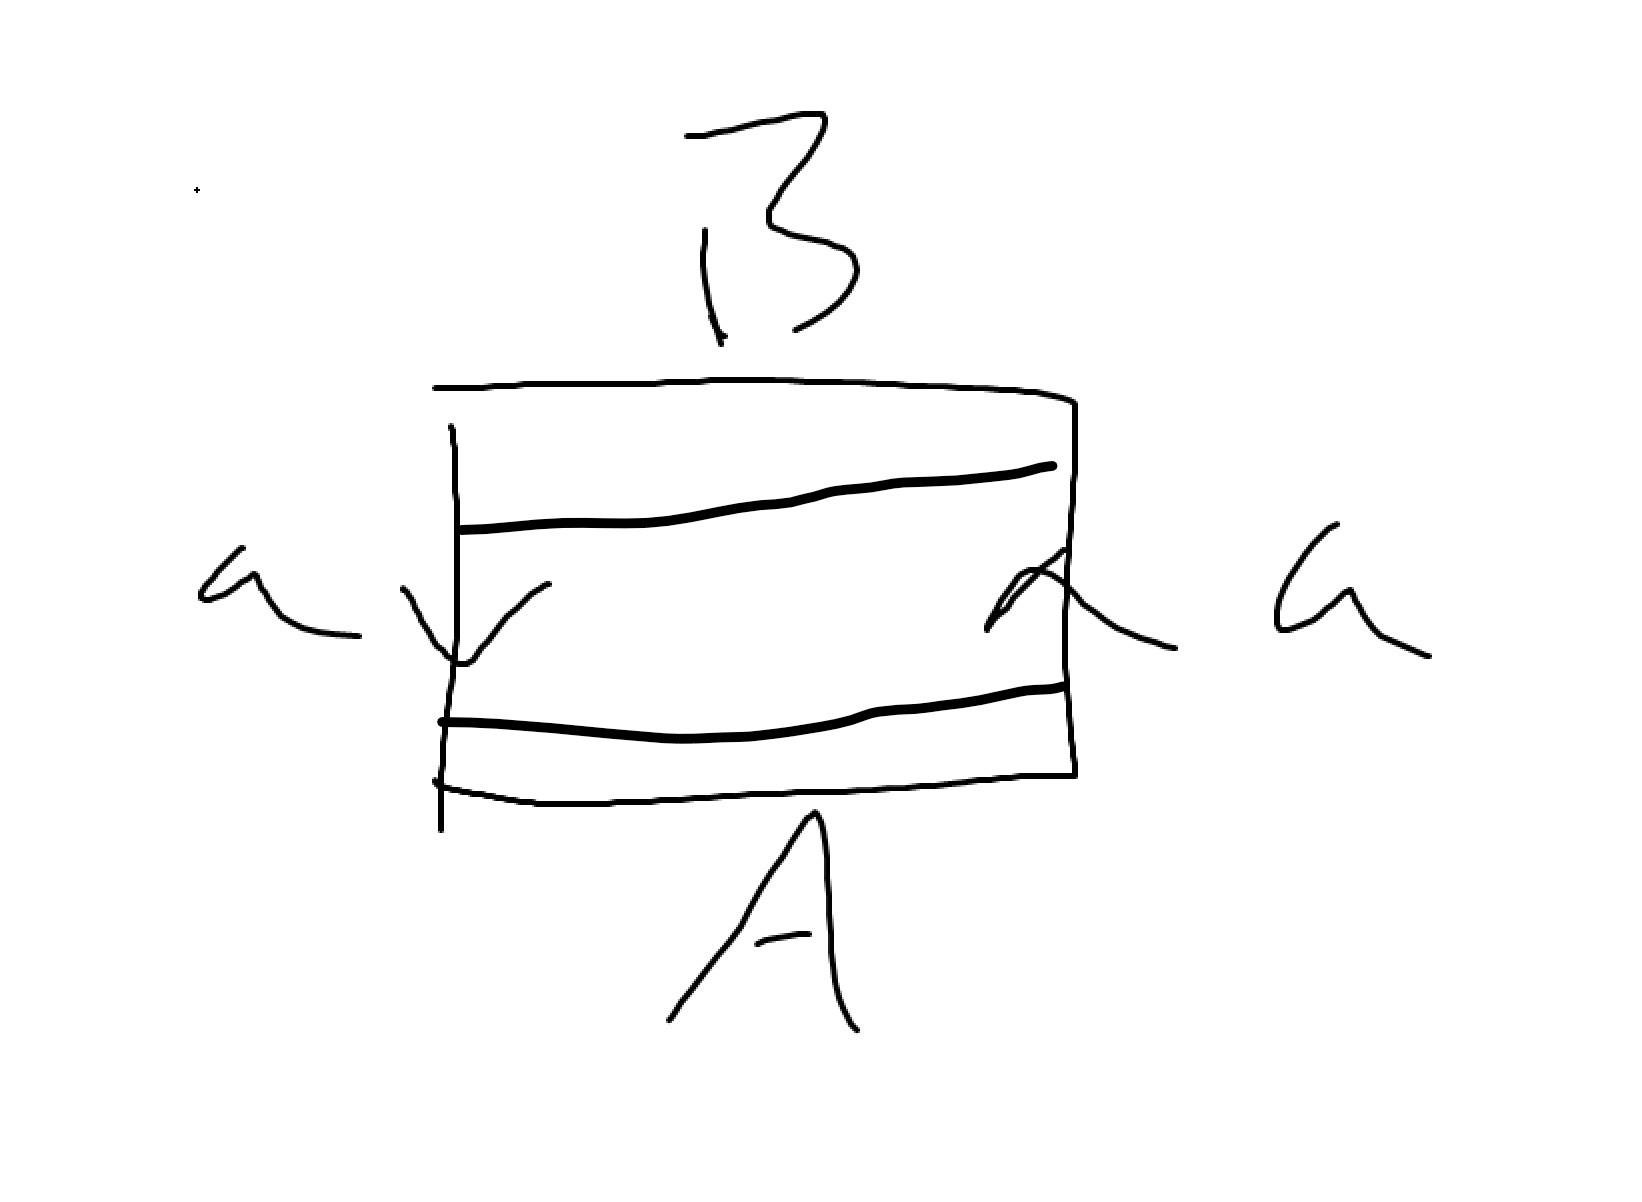
\includegraphics[scale=\linewidth]{homework/mobiusstrip.png}


\end{document}